\subsection{The Heat Equation}
Fourier Analysis was first discovered when Joseph Fourier first developed the Heat Equation. The Heat Equation models the flow of heat along a certain heat profile over time. In this example, a 1D solution will be derived and solved.

\subsubsection{Brief Derivation}
\noindent
Let us define a rod with the following assumptions:
\begin{itemize}
    \item The rod is of length \(L\) and is composed of an homogenous material with a heat diffusion coefficient \( \alpha^2 \).
    \item The rod is perfectly insulated along the Y and Z axes. Thus, heat can only flow along the X axis of the rod.
    \item The rod is thin enough such that the temperature of the rod at any cross-section is uniform.
    \item The rod is initially at a uniform temperature \(u(x,0) = f(x)\). Thus, the rod temperature at position \(x\) at time \(t\) is \(u(x,t)\).
\end{itemize}

% TODO: Is it worth it to actually derive the heat equation? It is beyond the scope of this paper.

\noindent
Thus, the heat equation in one dimension is defined as follows:
\begin{equation} \label{eq:heat_equation}
    \frac{\partial u}{\partial t} = \alpha^2 \nabla^2 u = \alpha^2 \frac{\partial^2 u}{\partial x^2}
\end{equation}

\noindent
Or in subscript notation,
\begin{equation} \label{eq:heat_equation_subscript}
    u_t = \alpha^2 u_{xx}
\end{equation}

\subsubsection{Application of the Fourier Transform}
Since \(u(x,t)\) is defined as the temperature of the rod at position \(x\) and time \(t\), we can apply the Fourier Transform to \(u(x,t)\) with respect to position \(x\) to reduce the \cref{eq:heat_equation_subscript} PDE into an ODE. Thus, let \(U(\kappa,t)\) be the Fourier Transform of \(u(x,t)\) with respect to \(x\).

\vspace{5mm}
\noindent
Taking the Fourier Transform of \cref{eq:heat_equation_subscript} with respect to \(x\),
\begin{equation}
    \mathcal{F} \left\{ u_t \right\} = \mathcal{F} \left\{ \alpha^2 u_{xx} \right\}
\end{equation}

\noindent
Using \cref{fourier_scaling},
\begin{equation}
    \mathcal{F} \left\{ u_t \right\} = \alpha^2 \mathcal{F} \left\{ u_{xx} \right\}
\end{equation}

\noindent
Using \cref{fourier_derivative},
\begin{align}
    \mathcal{F} \left\{ \frac{\partial^2 u(x, t)}{\partial x^2} \right\} & = i \kappa \mathcal{F} \left\{ \frac{\partial u(x, t)}{\partial x} \right\} \\
    & = -\kappa^2 \mathcal{F}\{ u(x, t) \} \\
    & = -\kappa^2 U
\end{align}

\noindent
Therefore,
\begin{align}
    \mathcal{F} \left\{ u_t \right\} &= -\alpha^2 \kappa^2 U \\
    \frac{dU}{dt} &= -\alpha^2 \kappa^2 U \label{eq:heat_equation_fourier}
\end{align}

\subsubsection{Boundary Conditions} % TODO: Add boundary conditions to the heat equation.

\subsubsection{Numerical Solution to Heat Equation} % TODO: Link the Python code for this numerical integration in the appendix.
\cref{eq:heat_equation_fourier} is a decoupled ODE that can be easily numerically integrated. A numerical solution to \cref{eq:heat_equation_fourier} using a fifth-order Runge-Kutta approximation in Python is presented below:

\begin{figure}[H]
    \centering
    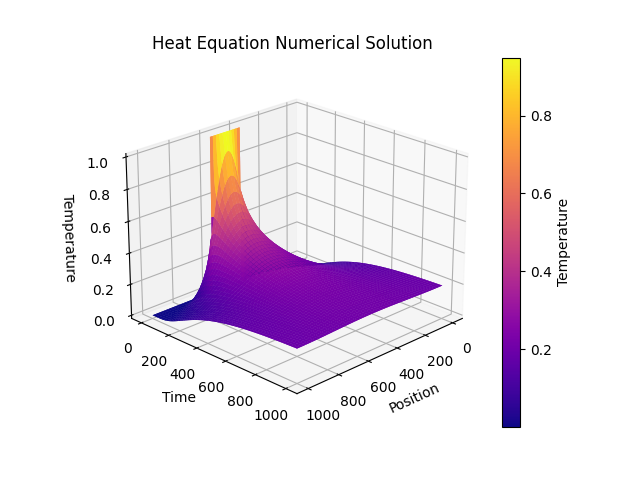
\includegraphics[width=110mm,height=\textheight,keepaspectratio]{images/heat_equation_numerical.png}
    \caption{Using a simple square waveform as the initial temperature function of the rod, this plot shows the temperature change along \(x\) and \(t\) by performing a numerical integration of \cref{eq:heat_equation_fourier}.}
    \label{fig:heat_equation_numerical}
\end{figure}

% \subsubsection{Analytical Solution to Heat Equation} 
% This is a maybe section. Possibly replace this section with a section on the applicability of the Fourier Transform to reduce PDEs to ODEs...?